\documentclass{article}

\usepackage[most]{tcolorbox}
\usepackage{physics}
\usepackage{graphicx}
\usepackage{float}
\usepackage{amsmath}
\usepackage{amssymb}


\usepackage[utf8]{inputenc}
\usepackage[a4paper, margin=1in]{geometry} % Controla los márgenes
\usepackage{titling}

\title{Clase 12 }
\author{Manuel Garcia.}
\date{\today}

\renewcommand{\maketitlehooka}{%
  \centering
  \vspace*{0.05cm} % Espacio vertical antes del título
}

\renewcommand{\maketitlehookd}{%
  \vspace*{2cm} % Espacio vertical después de la fecha
}

\newcommand{\caja}[3]{%
  \begin{tcolorbox}[colback=#1!5!white,colframe=#1!25!black,title=#2]
    #3
  \end{tcolorbox}%
}

\begin{document}
\maketitle

\section{Oscilador armonico }
\begin{gather*}
  a = \sqrt{\frac{m \omega}{2 \hbar }} \left(x + i \frac{p }{m \omega}\right) \qquad \qquad a ^ {\dag } = \sqrt{\frac{m \omega }{2 \hbar }} \left(x - i \frac{p }{m \omega}\right) \\
  N = a ^ {\dag } a = \frac{H }{\hbar  \omega }- \frac{1}{2} \qquad \qquad H = \frac{p ^2}{2m } + \frac{1}{2}m \omega ^2 x ^2 = \left(N + \frac{1}{2}\right)\hbar \omega\\
  N \ket{n } =  n \ket{n } \qquad n = 0,1,2,...\\
  a \ket{n } =  \sqrt{n } \ket{n -1 }\qquad a ^ {\dag } \ket{n } = \sqrt{n + 1 } \ket{n + 1 }
\end{gather*}
\begin{gather*}
  \bra{o }x \ket{o } = \int_{-\infty}^{\infty} dx \psi_0^*(x) x \psi_0 (x)  = \int_{- \infty}^{\infty}dx \underset{par }{[\psi_0(x)]^2} \underset{impar }{x}  = 0 
\end{gather*}

\begin{figure}[H]
  \begin{center}
    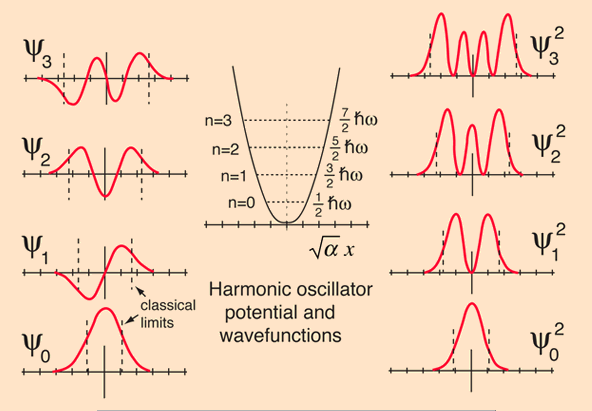
\includegraphics[width=0.5\textwidth]{wave_function.png}
  \end{center}
\end{figure}
\begin{gather*}
  \psi_0 = c_0 e ^ {- \frac{x ^2}{2 \bar x ^2}} \qquad \qquad \psi_1 = c_1 x e ^ {- \frac{x ^2 }{2 \bar x ^2}}
\end{gather*}

En fisica se dice \textbf{PAR: paridad positiva } e \textbf{IMPAR: paridad negativa}.

Como $ \psi_1  $ es lo mismo que $ \psi_0  $ pero con un x multiplicandola tenemos que: 
\begin{gather*}
  \bra{1 }x \ket{1 } = \int_{-\infty}^{\infty}\psi_1^* (x) x \psi_1(x)= 0   
\end{gather*}

Mas ejemplos: 
\begin{gather*}
  \bra{3 }x \ket{1 } = 0\\
  \bra{2 }x \ket{0 } = 0  
\end{gather*}

Qué sucede con el valor esperado del momentum? 
\begin{gather*}
  \bra{0 }p \ket{0 } = - i \hbar \int_{-\infty}^{\infty} dx \underset{par }{\psi_0^*(x) }\underset{impar }{\frac{d  }{d x }  } \underset{par }{\psi_0 (x) } = 0 \\
  \bra{n }p \ket{n } = 0  
\end{gather*}

Hay casos donde no da cero, por ejemplo: 
\begin{gather*}
  \bra{1 }x \ket{0 } = \int_{-\infty}^{\infty} dx \psi_1^* x \psi_0(x)
\end{gather*}

despejando de $ a  $ y $ a ^ {\dag } $ obtenemos que: 
\begin{gather*}
  x = c_1 a + c_2 a ^ {\dag } \qquad \qquad p = d_1 a + d_2 a ^ {\dag }
\end{gather*}
tanto $ x  $ como $ p  $ están conformados por un coeficiente de bajada y un coeficiente de subida.

\hfill

Aplicando esto al cambio de peldaño de 4 a 1 obtenemos:
\begin{gather*}
  \bra{4 }x \ket{1 } = 0   
\end{gather*}

En resumen si tenemos un cambio de peldaño de 1 va a ser diferente de 0 pero si tenemos un cambio de peldaño de mas de 1 nos va a dar 0.

\caja{red}{}{
  \begin{gather*}
    \bra{n ' }x \ket{n } = \sqrt{\frac{\hbar }{2m \omega }}  (\sqrt{n } \delta _{n ', n-1 } + \sqrt{n + 1 } \delta _{n ' , n + 1 } )  \\
    \bra{n ' }p \ket{n } = i \sqrt{\frac{m \hbar  \omega }{2}} (- \sqrt{n } \delta _{n ' , n-1 } + \sqrt{n + 1 } \delta _{n ' , n + 1 } ) 
  \end{gather*}
}

Qué sucede si queremos hallar $ \bra{n' }x \ket{n }  $?
\begin{gather*}
  \bra{n'}x \ket{n } = \int_{- \infty}^{\infty} dx \psi _{n' } ^ {* }(x) x ^2 \psi_n (x)   
\end{gather*}
Según el libro: 
\caja{red}{}{
  $ x ^2 = \frac{\hbar }{2m \omega} (a ^2 + a ^ {\dag 2 } + a ^ {\dag } a + a a ^ {\dag}) $ y tenemos que $ a a ^ {\dag } - a ^ {\dag }a = 1 \rightarrow a a ^ {\dag } = 1 + a ^ {\dag }a  $, por lo tanto: 
  \begin{gather*}
    x ^2 = \frac{\hbar }{2m \omega} (a ^2 + a ^ {\dag 2 } + 2N +1)
  \end{gather*}
}

\caja{black}{Tarea }{
  Calcular la transformada de fourier de 
  \begin{gather*}
    \psi_p(x) = N e ^ {i \frac{p x }{\hbar }} = N\left[\cos{\frac{px }{\hbar }} + i \sin{\frac{px }{\hbar }}\right] 
  \end{gather*}
}

\hfill 

\hfill 

\begin{gather*}
  H = \frac{p ^2}{2 m } + \frac{1}{2} m \omega ^2 x ^2\\
  H \ket{\psi } = E \ket{\psi } \qquad \qquad \bra{x}\ket{\psi } = \psi(x) \\
  \bra{x }H \ket{\psi } = E \bra{x }\ket{\psi} \\
  \bra{x }p ^2\ket{\psi} = - \hbar ^2 \frac{d ^2  }{d x^2}\psi(x) 
\end{gather*}

Ecuacion de schrodinger: 
\begin{gather*}
  - \frac{\hbar  ^2}{2m }\frac{d ^2\psi(x)  }{d x ^2} + \frac{1}{2}m \omega ^2 x ^2 \psi(x) = E \psi(x) 
\end{gather*}

tenemos que $ \bar x  = \sqrt{\frac{\hbar }{m \omega}}  $ y $ \xi = \frac{x }{\bar x } $:
\begin{gather*}
  \frac{d ^2  }{d \xi ^2} \psi(\xi) - \xi^2 \psi(\xi ) + \frac{2E }{\hbar \omega} \psi(\xi) = 0 
\end{gather*}

Como el segundo termino tiene $ \xi^2  $ es un termino mucho mas grande que el tercero por lo tanto podemos despreciar el tercero.

\end{document}
